% Options for packages loaded elsewhere
\PassOptionsToPackage{unicode}{hyperref}
\PassOptionsToPackage{hyphens}{url}
\PassOptionsToPackage{dvipsnames,svgnames,x11names}{xcolor}
%
\documentclass[
  us-letterpaper,
  DIV=11,
  numbers=noendperiod]{scrreprt}

\usepackage{amsmath,amssymb}
\usepackage{iftex}
\ifPDFTeX
  \usepackage[T1]{fontenc}
  \usepackage[utf8]{inputenc}
  \usepackage{textcomp} % provide euro and other symbols
\else % if luatex or xetex
  \usepackage{unicode-math}
  \defaultfontfeatures{Scale=MatchLowercase}
  \defaultfontfeatures[\rmfamily]{Ligatures=TeX,Scale=1}
\fi
\usepackage{lmodern}
\ifPDFTeX\else  
    % xetex/luatex font selection
\fi
% Use upquote if available, for straight quotes in verbatim environments
\IfFileExists{upquote.sty}{\usepackage{upquote}}{}
\IfFileExists{microtype.sty}{% use microtype if available
  \usepackage[]{microtype}
  \UseMicrotypeSet[protrusion]{basicmath} % disable protrusion for tt fonts
}{}
\makeatletter
\@ifundefined{KOMAClassName}{% if non-KOMA class
  \IfFileExists{parskip.sty}{%
    \usepackage{parskip}
  }{% else
    \setlength{\parindent}{0pt}
    \setlength{\parskip}{6pt plus 2pt minus 1pt}}
}{% if KOMA class
  \KOMAoptions{parskip=half}}
\makeatother
\usepackage{xcolor}
\setlength{\emergencystretch}{3em} % prevent overfull lines
\setcounter{secnumdepth}{5}
% Make \paragraph and \subparagraph free-standing
\makeatletter
\ifx\paragraph\undefined\else
  \let\oldparagraph\paragraph
  \renewcommand{\paragraph}{
    \@ifstar
      \xxxParagraphStar
      \xxxParagraphNoStar
  }
  \newcommand{\xxxParagraphStar}[1]{\oldparagraph*{#1}\mbox{}}
  \newcommand{\xxxParagraphNoStar}[1]{\oldparagraph{#1}\mbox{}}
\fi
\ifx\subparagraph\undefined\else
  \let\oldsubparagraph\subparagraph
  \renewcommand{\subparagraph}{
    \@ifstar
      \xxxSubParagraphStar
      \xxxSubParagraphNoStar
  }
  \newcommand{\xxxSubParagraphStar}[1]{\oldsubparagraph*{#1}\mbox{}}
  \newcommand{\xxxSubParagraphNoStar}[1]{\oldsubparagraph{#1}\mbox{}}
\fi
\makeatother

\usepackage{color}
\usepackage{fancyvrb}
\newcommand{\VerbBar}{|}
\newcommand{\VERB}{\Verb[commandchars=\\\{\}]}
\DefineVerbatimEnvironment{Highlighting}{Verbatim}{commandchars=\\\{\}}
% Add ',fontsize=\small' for more characters per line
\usepackage{framed}
\definecolor{shadecolor}{RGB}{241,243,245}
\newenvironment{Shaded}{\begin{snugshade}}{\end{snugshade}}
\newcommand{\AlertTok}[1]{\textcolor[rgb]{0.68,0.00,0.00}{#1}}
\newcommand{\AnnotationTok}[1]{\textcolor[rgb]{0.37,0.37,0.37}{#1}}
\newcommand{\AttributeTok}[1]{\textcolor[rgb]{0.40,0.45,0.13}{#1}}
\newcommand{\BaseNTok}[1]{\textcolor[rgb]{0.68,0.00,0.00}{#1}}
\newcommand{\BuiltInTok}[1]{\textcolor[rgb]{0.00,0.23,0.31}{#1}}
\newcommand{\CharTok}[1]{\textcolor[rgb]{0.13,0.47,0.30}{#1}}
\newcommand{\CommentTok}[1]{\textcolor[rgb]{0.37,0.37,0.37}{#1}}
\newcommand{\CommentVarTok}[1]{\textcolor[rgb]{0.37,0.37,0.37}{\textit{#1}}}
\newcommand{\ConstantTok}[1]{\textcolor[rgb]{0.56,0.35,0.01}{#1}}
\newcommand{\ControlFlowTok}[1]{\textcolor[rgb]{0.00,0.23,0.31}{\textbf{#1}}}
\newcommand{\DataTypeTok}[1]{\textcolor[rgb]{0.68,0.00,0.00}{#1}}
\newcommand{\DecValTok}[1]{\textcolor[rgb]{0.68,0.00,0.00}{#1}}
\newcommand{\DocumentationTok}[1]{\textcolor[rgb]{0.37,0.37,0.37}{\textit{#1}}}
\newcommand{\ErrorTok}[1]{\textcolor[rgb]{0.68,0.00,0.00}{#1}}
\newcommand{\ExtensionTok}[1]{\textcolor[rgb]{0.00,0.23,0.31}{#1}}
\newcommand{\FloatTok}[1]{\textcolor[rgb]{0.68,0.00,0.00}{#1}}
\newcommand{\FunctionTok}[1]{\textcolor[rgb]{0.28,0.35,0.67}{#1}}
\newcommand{\ImportTok}[1]{\textcolor[rgb]{0.00,0.46,0.62}{#1}}
\newcommand{\InformationTok}[1]{\textcolor[rgb]{0.37,0.37,0.37}{#1}}
\newcommand{\KeywordTok}[1]{\textcolor[rgb]{0.00,0.23,0.31}{\textbf{#1}}}
\newcommand{\NormalTok}[1]{\textcolor[rgb]{0.00,0.23,0.31}{#1}}
\newcommand{\OperatorTok}[1]{\textcolor[rgb]{0.37,0.37,0.37}{#1}}
\newcommand{\OtherTok}[1]{\textcolor[rgb]{0.00,0.23,0.31}{#1}}
\newcommand{\PreprocessorTok}[1]{\textcolor[rgb]{0.68,0.00,0.00}{#1}}
\newcommand{\RegionMarkerTok}[1]{\textcolor[rgb]{0.00,0.23,0.31}{#1}}
\newcommand{\SpecialCharTok}[1]{\textcolor[rgb]{0.37,0.37,0.37}{#1}}
\newcommand{\SpecialStringTok}[1]{\textcolor[rgb]{0.13,0.47,0.30}{#1}}
\newcommand{\StringTok}[1]{\textcolor[rgb]{0.13,0.47,0.30}{#1}}
\newcommand{\VariableTok}[1]{\textcolor[rgb]{0.07,0.07,0.07}{#1}}
\newcommand{\VerbatimStringTok}[1]{\textcolor[rgb]{0.13,0.47,0.30}{#1}}
\newcommand{\WarningTok}[1]{\textcolor[rgb]{0.37,0.37,0.37}{\textit{#1}}}

\providecommand{\tightlist}{%
  \setlength{\itemsep}{0pt}\setlength{\parskip}{0pt}}\usepackage{longtable,booktabs,array}
\usepackage{calc} % for calculating minipage widths
% Correct order of tables after \paragraph or \subparagraph
\usepackage{etoolbox}
\makeatletter
\patchcmd\longtable{\par}{\if@noskipsec\mbox{}\fi\par}{}{}
\makeatother
% Allow footnotes in longtable head/foot
\IfFileExists{footnotehyper.sty}{\usepackage{footnotehyper}}{\usepackage{footnote}}
\makesavenoteenv{longtable}
\usepackage{graphicx}
\makeatletter
\def\maxwidth{\ifdim\Gin@nat@width>\linewidth\linewidth\else\Gin@nat@width\fi}
\def\maxheight{\ifdim\Gin@nat@height>\textheight\textheight\else\Gin@nat@height\fi}
\makeatother
% Scale images if necessary, so that they will not overflow the page
% margins by default, and it is still possible to overwrite the defaults
% using explicit options in \includegraphics[width, height, ...]{}
\setkeys{Gin}{width=\maxwidth,height=\maxheight,keepaspectratio}
% Set default figure placement to htbp
\makeatletter
\def\fps@figure{htbp}
\makeatother
% definitions for citeproc citations
\NewDocumentCommand\citeproctext{}{}
\NewDocumentCommand\citeproc{mm}{%
  \begingroup\def\citeproctext{#2}\cite{#1}\endgroup}
\makeatletter
 % allow citations to break across lines
 \let\@cite@ofmt\@firstofone
 % avoid brackets around text for \cite:
 \def\@biblabel#1{}
 \def\@cite#1#2{{#1\if@tempswa , #2\fi}}
\makeatother
\newlength{\cslhangindent}
\setlength{\cslhangindent}{1.5em}
\newlength{\csllabelwidth}
\setlength{\csllabelwidth}{3em}
\newenvironment{CSLReferences}[2] % #1 hanging-indent, #2 entry-spacing
 {\begin{list}{}{%
  \setlength{\itemindent}{0pt}
  \setlength{\leftmargin}{0pt}
  \setlength{\parsep}{0pt}
  % turn on hanging indent if param 1 is 1
  \ifodd #1
   \setlength{\leftmargin}{\cslhangindent}
   \setlength{\itemindent}{-1\cslhangindent}
  \fi
  % set entry spacing
  \setlength{\itemsep}{#2\baselineskip}}}
 {\end{list}}
\usepackage{calc}
\newcommand{\CSLBlock}[1]{\hfill\break\parbox[t]{\linewidth}{\strut\ignorespaces#1\strut}}
\newcommand{\CSLLeftMargin}[1]{\parbox[t]{\csllabelwidth}{\strut#1\strut}}
\newcommand{\CSLRightInline}[1]{\parbox[t]{\linewidth - \csllabelwidth}{\strut#1\strut}}
\newcommand{\CSLIndent}[1]{\hspace{\cslhangindent}#1}


\KOMAoption{captions}{tableheading}
\makeatletter
\@ifpackageloaded{bookmark}{}{\usepackage{bookmark}}
\makeatother
\makeatletter
\@ifpackageloaded{caption}{}{\usepackage{caption}}
\AtBeginDocument{%
\ifdefined\contentsname
  \renewcommand*\contentsname{Tabla de contenidos}
\else
  \newcommand\contentsname{Tabla de contenidos}
\fi
\ifdefined\listfigurename
  \renewcommand*\listfigurename{Listado de Figuras}
\else
  \newcommand\listfigurename{Listado de Figuras}
\fi
\ifdefined\listtablename
  \renewcommand*\listtablename{Listado de Tablas}
\else
  \newcommand\listtablename{Listado de Tablas}
\fi
\ifdefined\figurename
  \renewcommand*\figurename{Figura}
\else
  \newcommand\figurename{Figura}
\fi
\ifdefined\tablename
  \renewcommand*\tablename{Tabla}
\else
  \newcommand\tablename{Tabla}
\fi
}
\@ifpackageloaded{float}{}{\usepackage{float}}
\floatstyle{ruled}
\@ifundefined{c@chapter}{\newfloat{codelisting}{h}{lop}}{\newfloat{codelisting}{h}{lop}[chapter]}
\floatname{codelisting}{Listado}
\newcommand*\listoflistings{\listof{codelisting}{Listado de Listados}}
\makeatother
\makeatletter
\makeatother
\makeatletter
\@ifpackageloaded{caption}{}{\usepackage{caption}}
\@ifpackageloaded{subcaption}{}{\usepackage{subcaption}}
\makeatother

\ifLuaTeX
\usepackage[bidi=basic]{babel}
\else
\usepackage[bidi=default]{babel}
\fi
\babelprovide[main,import]{spanish}
% get rid of language-specific shorthands (see #6817):
\let\LanguageShortHands\languageshorthands
\def\languageshorthands#1{}
\ifLuaTeX
  \usepackage{selnolig}  % disable illegal ligatures
\fi
\usepackage{bookmark}

\IfFileExists{xurl.sty}{\usepackage{xurl}}{} % add URL line breaks if available
\urlstyle{same} % disable monospaced font for URLs
\hypersetup{
  pdftitle={Análisis Futbol},
  pdflang={es-MX},
  colorlinks=true,
  linkcolor={blue},
  filecolor={Maroon},
  citecolor={Blue},
  urlcolor={Blue},
  pdfcreator={LaTeX via pandoc}}


\title{Análisis Futbol}
\author{}
\date{2024-02-14}

\begin{document}
\maketitle

\renewcommand*\contentsname{Tabla de contenidos}
{
\hypersetup{linkcolor=}
\setcounter{tocdepth}{2}
\tableofcontents
}

\bookmarksetup{startatroot}

\chapter*{Introducción}\label{introducciuxf3n}
\addcontentsline{toc}{chapter}{Introducción}

\markboth{Introducción}{Introducción}

Este trabajo está basado en los trabajos: Van Roy, Yang, et~al. (2021) y
Van Roy, Robberechts, et~al. (2021).

Para la construcción del Proceso de Decisión de Markov (MDP) del
planteado en este trabajo, primero debemos recordar algunas reglas
durante un partido de fútbol para aquellos que no las conozcan y también
haremos algunas puntualizaciones respecto a la naturaleza de un partido.

Además se darán algunas hipótesis para simplificar el modelo sin pérder
la escencia del juego.

Un partido de fútbol se componen de 2 equipos con 11 jugadores cada uno,
un balón y un arbitro (o un grupo de arbitros). Los equipos se
posicionan dentro de un terreno de juego que consta de 2 porterias (una
para cada equipo), el objetivo de cada equipo es anotar un gol (que el
balón ingrese por completo dentro de la porteria) en la portería del
equipo contrario. Por cada gol un equipo recibe lo que sería 1 punto, al
final del partido el equipo que anote más goles gana y en caso de anotar
la misma cantidad se considera empate.

{[}Agregar campo de juego con 11 jugadores para cada equipo, Equipo A y
Equipo B{]}

Para anotar un gol cada jugador puede tocar el balón con cualquier parte
del cuerpo salvo el brazo, sin embargo, de los 11 jugadores de cada
equipo hay un futbolista que puede tomar el balón con las manos dentro
de las áreas marcadas alrededor de las porterias, a este jugador se le
conoce como portero.

Un partido consta de 90 minutos divididos en 2 partes de 45 minutos.

Explicadas las reglas principales vamos a familiarizarnos con el
desarrollo de un partido.

Si bien no existen reglas escritas sobre como se deban acomodar los 11
jugadores en el campo, durante la historia siempre se han acomodado de
la siguiente forma:

\begin{itemize}
\tightlist
\item
  El portero siempre se mantiene dentro del área y lo más cercano a la
  portería.
\item
  Existe un primer grupo llamados defensas que se acomodan delante del
  portero y son los encargados que el equipo contrario no marque gol.
\item
  Existe un segundo grupo llamados mediocampistas que se acomodan
  delante de los defensas y que su función es trasladar el balón de los
  defensas hacia la portería rival.
\item
  Existe un tercer grupo llamados delanteros que son los encargados de
  recibir los balones de los mediocampistas y tratar de anotar gol.
\end{itemize}

{[}Agregar campo de juego con 4-3-3{]}

El problema principal al que nos enfrentamos y por lo cuál el fútbol es
tan dificil de analizar es porque las descripciones anteriores son muy
generales y muchas veces no se cumplen. Es decir, podemos tener a un
defensa o un mediocampista metiendo goles sin necesidad de los
delanteros, podemos tener mediocampistas defendiendo o se puede anotar
un gol pasando directamente de los defensas o el portero hasta los
delanteros. En cuestión de dinámica casi todo está permitido, esto no
quiere decir que suceda, sin embargo es muy complicado analizar de forma
mecanica cada decisión de los fútbolistas.

Aún así podemos enlistar ciertas situaciones que no son comunes que
pasen y por tanto para nuestro modelo las vamos a ignorar:

\begin{itemize}
\tightlist
\item
  No se anotan goles desde la primera mitad de campo (desde la portería
  propia hasta el medio campo).
\item
  Los porteros no anotan goles.
\item
  La única forma de anotar gol es mediante una acción que llamamos
  tiros.
\item
  Cada equipo tiene 11 jugadores.
\end{itemize}

También durante el desarrollo de un partido hay múltiples acciones que
puede realizar un futbolista, a continuación enlistamos algunas de las
acciones:

\begin{itemize}
\tightlist
\item
  pase : Golpear el balón con el pie, cabeza o alguna otra parte del
  cuerpo con intención que el balón llegue a un jugador del mismo
  equipo.
\end{itemize}

\url{https://www.youtube.com/watch?v=f-Bw-UaVV4U&ab_channel=SportsHD}

\begin{itemize}
\tightlist
\item
  tiro : Golpear el balón con el pie, cabeza o alguna otra parte del
  cuerpo con intención que el balón ingrese en la porteria contraria.
\end{itemize}

\url{https://www.youtube.com/watch?v=si1RC4w-FAI&ab_channel=90Minutes}

\begin{itemize}
\tightlist
\item
  regate : Mover el balón de forma que el jugador rival no me lo quite y
  me haga avanzar o terminar en una posición favorable.
\end{itemize}

\url{https://www.youtube.com/watch?v=mathV4xFUX8&ab_channel=VSVHD}

\begin{itemize}
\tightlist
\item
  centro : Golpear el balón con el pie, cabeza o alguna otra parte del
  cuerpo con intención que el balón llegue por el aire a un jugador del
  mismo equipo.
\end{itemize}

\url{https://www.youtube.com/watch?v=-nI94rkcOwk&t=11s&ab_channel=rom7ooo}

Existen muchas más acciones que puede realizar un futbolista, sin
embargo las enlistadas anteriormente son las más comunes y muchas se
desprenden de ellas.

Con todo lo anterior podemos dejar claro cuál es el próposito del
proyecto.

Como mencionamos lo más importante durante un partido son los goles, hay
que marcar goles y evitar que nos marquen gol. En este proyecto nos
centramos en la parte ofensiva, es decir marcar goles. De esta forma
nuestro proposito es el de encontrar la mejor forma de mover el balón
por el campo que nos haga marcar un gol.

Para lograr esto se van a hacer algunas hipótesis:

\begin{itemize}
\tightlist
\item
  El campo se divide en 3 secciones iguales: Defensa, Mediocampo,
  Delantera.
\item
  Solo se consideran 3 acciones: pase, tiro, regate.
\item
  Los jugadores toman decisiones coherentes.
\item
  No se consideran: fuera de juego, tiros libres, penales, saques de
  banda.
\end{itemize}

Llamaremos jugada a una serie de acciones y puntulizar que:

\begin{itemize}
\tightlist
\item
  Una jugada puede comenzar en cualquier parte del campo.
\item
  Una jugada termina cuando realizamos un tiro o cuando perdemos el
  balón.
\end{itemize}

\bookmarksetup{startatroot}

\chapter{Formulación}\label{formulaciuxf3n}

El Proceso de Decisión de Markov se compone de los siguientes elementos:

\begin{itemize}
\tightlist
\item
  El conjunto de estados estará conformado por las siguientes tres
  divisiones del campo
\end{itemize}

\begin{Shaded}
\begin{Highlighting}[]
\ImportTok{import}\NormalTok{ numpy }\ImportTok{as}\NormalTok{ np }
\ImportTok{import}\NormalTok{ pandas }\ImportTok{as}\NormalTok{ pd}
\ImportTok{import}\NormalTok{ matplotlib.pyplot }\ImportTok{as}\NormalTok{ plt }
\ImportTok{from}\NormalTok{ matplotlib.colors }\ImportTok{import}\NormalTok{ to\_rgba}
\ImportTok{from}\NormalTok{ urllib.request }\ImportTok{import}\NormalTok{ urlopen}
\ImportTok{from}\NormalTok{ mplsoccer }\ImportTok{import}\NormalTok{ Pitch, FontManager, add\_image}
\ImportTok{from}\NormalTok{ PIL }\ImportTok{import}\NormalTok{ Image}

\NormalTok{pitch }\OperatorTok{=}\NormalTok{ Pitch(line\_color}\OperatorTok{=}\StringTok{\textquotesingle{}black\textquotesingle{}}\NormalTok{,linewidth}\OperatorTok{=}\DecValTok{1}\NormalTok{)}
\NormalTok{fig, ax }\OperatorTok{=}\NormalTok{ pitch.draw()}
\NormalTok{pitch.lines(}\DecValTok{40}\NormalTok{,}\DecValTok{0}\NormalTok{,}\DecValTok{40}\NormalTok{,}\DecValTok{80}\NormalTok{,color }\OperatorTok{=} \StringTok{\textquotesingle{}gray\textquotesingle{}}\NormalTok{, linewidth }\OperatorTok{=} \DecValTok{1}\NormalTok{, ax}\OperatorTok{=}\NormalTok{ax, linestyle }\OperatorTok{=} \StringTok{\textquotesingle{}{-}{-}\textquotesingle{}}\NormalTok{)}

\NormalTok{pitch.lines(}\DecValTok{80}\NormalTok{,}\DecValTok{0}\NormalTok{,}\DecValTok{80}\NormalTok{,}\DecValTok{80}\NormalTok{,color }\OperatorTok{=} \StringTok{\textquotesingle{}gray\textquotesingle{}}\NormalTok{, linewidth }\OperatorTok{=} \DecValTok{1}\NormalTok{, ax}\OperatorTok{=}\NormalTok{ax, linestyle }\OperatorTok{=} \StringTok{\textquotesingle{}{-}{-}\textquotesingle{}}\NormalTok{)}

\NormalTok{pitch.annotate(text}\OperatorTok{=}\StringTok{\textquotesingle{}$C\_1$\textquotesingle{}}\NormalTok{,xytext}\OperatorTok{=}\NormalTok{(}\DecValTok{10}\NormalTok{,}\DecValTok{10}\NormalTok{),xy}\OperatorTok{=}\NormalTok{(}\DecValTok{84}\NormalTok{,}\DecValTok{45}\NormalTok{),ax}\OperatorTok{=}\NormalTok{ax)}
\NormalTok{pitch.annotate(text}\OperatorTok{=}\StringTok{\textquotesingle{}$C\_2$\textquotesingle{}}\NormalTok{,xytext}\OperatorTok{=}\NormalTok{(}\DecValTok{50}\NormalTok{,}\DecValTok{10}\NormalTok{),xy}\OperatorTok{=}\NormalTok{(}\DecValTok{84}\NormalTok{,}\DecValTok{45}\NormalTok{),ax}\OperatorTok{=}\NormalTok{ax)}
\NormalTok{pitch.annotate(text}\OperatorTok{=}\StringTok{\textquotesingle{}$C\_3$\textquotesingle{}}\NormalTok{,xytext}\OperatorTok{=}\NormalTok{(}\DecValTok{90}\NormalTok{,}\DecValTok{10}\NormalTok{),xy}\OperatorTok{=}\NormalTok{(}\DecValTok{84}\NormalTok{,}\DecValTok{45}\NormalTok{),ax}\OperatorTok{=}\NormalTok{ax)}
\NormalTok{plt.show()}
\end{Highlighting}
\end{Shaded}

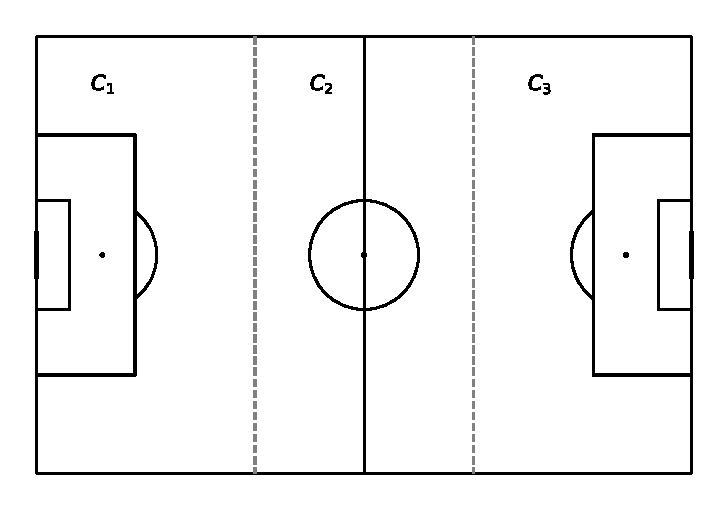
\includegraphics{formulacion_files/figure-pdf/cell-2-output-1.pdf}

Donde \(C_1,C_2,C_3\) representa que el balón se encuentre en alguna de
las tres divisiones.

Además se agregan tres estados absorbentes:

\begin{itemize}
\tightlist
\item
  \(L_p =\) pérdida de posesión del balón.
\item
  \(nG =\) realizar un tiro y que no termine en gol.
\item
  \(G =\) realizar un tiro y que termine en gol.
\end{itemize}

De esta forma el conjunto de estados \(\mathcal{S}\) queda como

\[
    \mathcal{S}=\{C_1,C_2,C_3,L_p,nG,G\}
\]

\begin{itemize}
\item
  El conjunto de acciones admisibles se considerarán 3 acciones que
  serán

  \begin{itemize}
  \tightlist
  \item
    \(t\) = tiro
  \item
    \(p\) = pase
  \item
    \(r\) = regate
  \end{itemize}

  De esta forma el conjunto de acciones queda como
  \[\mathcal{A} = \{t,p,r\}\]
\item
  Para las de transiciones haremos uso de las probabilidades de
  transición definidas de la siguiente forma: \[
   P:\mathcal{S}\times\mathcal{A}\times\mathcal{S} \to [0,1]
   \]

  Que se interpreta como la probabilidad de estar en un estado \(S_i\)
  realizar una acción \(a_k\) y terminar en un estado \(S_j\). Notemos
  que se aceptan los casos cuando \(i=j\) y más adelante se mostrará que
  algunas probabilidades serán 0.
\item
  La función de recompensa
  \(R:\mathcal{S}\times \mathcal{A}\times \mathcal{S}\to[0,1]\), será \[
    R(S_i,a_k,S_j)=\left\{\begin{array}{ccc}
                 1 & \text{si} & S_j=G  \\
                 0 & o.c. &
            \end{array}\right.
    \]
\end{itemize}

\bookmarksetup{startatroot}

\chapter{Dinámica del modelo}\label{dinuxe1mica-del-modelo}

En el contexto del fútbol llamamos \emph{jugada} a una sucesión de
acciones donde el balón se traslada desde un punto inicial donde el
equipo A tiene el balón hasta un punto final que puede ser: perder el
balón, tirar a puerta y no anotar gol o tirar y anotar gol.

\emph{Ejemplo: El balón comienza en el saque de meta del portero, el
portero da un pase a un defensa que se encuentra en el primer tercio,
que esté da un pase a un delantero que se encuentra en el tercer tercio
y al intentar un regate pierde el balón.}

En nuestro contexto se verá como el hecho de iniciar la sucesión de
acciones desde alguna sección \(C_i\) y terminar en alguno de los 3
estados absorbentes.

\emph{Ejemplo} \[
C_1\xrightarrow{p}C_1\xrightarrow{p}C_3\xrightarrow{r}L_p.
\]

\begin{Shaded}
\begin{Highlighting}[]
\ImportTok{import}\NormalTok{ numpy }\ImportTok{as}\NormalTok{ np }
\ImportTok{import}\NormalTok{ pandas }\ImportTok{as}\NormalTok{ pd}
\ImportTok{import}\NormalTok{ matplotlib.pyplot }\ImportTok{as}\NormalTok{ plt }
\ImportTok{from}\NormalTok{ mplsoccer }\ImportTok{import}\NormalTok{ Pitch, FontManager, add\_image}

\NormalTok{pitch }\OperatorTok{=}\NormalTok{ Pitch(line\_color}\OperatorTok{=}\StringTok{\textquotesingle{}black\textquotesingle{}}\NormalTok{,linewidth}\OperatorTok{=}\DecValTok{1}\NormalTok{)}
\NormalTok{fig, ax }\OperatorTok{=}\NormalTok{ pitch.draw()}
\NormalTok{pitch.lines(}\DecValTok{40}\NormalTok{,}\DecValTok{0}\NormalTok{,}\DecValTok{40}\NormalTok{,}\DecValTok{80}\NormalTok{,color }\OperatorTok{=} \StringTok{\textquotesingle{}gray\textquotesingle{}}\NormalTok{, linewidth }\OperatorTok{=} \DecValTok{1}\NormalTok{, ax}\OperatorTok{=}\NormalTok{ax, linestyle }\OperatorTok{=} \StringTok{\textquotesingle{}{-}{-}\textquotesingle{}}\NormalTok{)}

\NormalTok{pitch.lines(}\DecValTok{80}\NormalTok{,}\DecValTok{0}\NormalTok{,}\DecValTok{80}\NormalTok{,}\DecValTok{80}\NormalTok{,color }\OperatorTok{=} \StringTok{\textquotesingle{}gray\textquotesingle{}}\NormalTok{, linewidth }\OperatorTok{=} \DecValTok{1}\NormalTok{, ax}\OperatorTok{=}\NormalTok{ax, linestyle }\OperatorTok{=} \StringTok{\textquotesingle{}{-}{-}\textquotesingle{}}\NormalTok{)}

\NormalTok{pitch.annotate(text}\OperatorTok{=}\StringTok{\textquotesingle{}$C\_1$\textquotesingle{}}\NormalTok{,xytext}\OperatorTok{=}\NormalTok{(}\DecValTok{10}\NormalTok{,}\DecValTok{10}\NormalTok{),xy}\OperatorTok{=}\NormalTok{(}\DecValTok{84}\NormalTok{,}\DecValTok{45}\NormalTok{),ax}\OperatorTok{=}\NormalTok{ax)}
\NormalTok{pitch.annotate(text}\OperatorTok{=}\StringTok{\textquotesingle{}$C\_2$\textquotesingle{}}\NormalTok{,xytext}\OperatorTok{=}\NormalTok{(}\DecValTok{50}\NormalTok{,}\DecValTok{10}\NormalTok{),xy}\OperatorTok{=}\NormalTok{(}\DecValTok{84}\NormalTok{,}\DecValTok{45}\NormalTok{),ax}\OperatorTok{=}\NormalTok{ax)}
\NormalTok{pitch.annotate(text}\OperatorTok{=}\StringTok{\textquotesingle{}$C\_3$\textquotesingle{}}\NormalTok{,xytext}\OperatorTok{=}\NormalTok{(}\DecValTok{90}\NormalTok{,}\DecValTok{10}\NormalTok{),xy}\OperatorTok{=}\NormalTok{(}\DecValTok{84}\NormalTok{,}\DecValTok{45}\NormalTok{),ax}\OperatorTok{=}\NormalTok{ax)}

\NormalTok{pitch.scatter(}\DecValTok{0}\NormalTok{,}\DecValTok{40}\NormalTok{, color }\OperatorTok{=} \StringTok{\textquotesingle{}red\textquotesingle{}}\NormalTok{, ax}\OperatorTok{=}\NormalTok{ax)}
\NormalTok{pitch.scatter(}\DecValTok{24}\NormalTok{,}\DecValTok{62}\NormalTok{,color }\OperatorTok{=} \StringTok{\textquotesingle{}red\textquotesingle{}}\NormalTok{,ax}\OperatorTok{=}\NormalTok{ax)}
\NormalTok{pitch.scatter(}\DecValTok{84}\NormalTok{,}\DecValTok{45}\NormalTok{,color }\OperatorTok{=} \StringTok{\textquotesingle{}red\textquotesingle{}}\NormalTok{,ax}\OperatorTok{=}\NormalTok{ax)}

\NormalTok{pitch.arrows(}\DecValTok{0}\NormalTok{,}\DecValTok{40}\NormalTok{,}\DecValTok{24}\NormalTok{,}\DecValTok{62}\NormalTok{,color }\OperatorTok{=} \StringTok{\textquotesingle{}green\textquotesingle{}}\NormalTok{, width }\OperatorTok{=} \DecValTok{2}\NormalTok{,label }\OperatorTok{=} \StringTok{\textquotesingle{}Pase\textquotesingle{}}\NormalTok{, ax}\OperatorTok{=}\NormalTok{ax)}
\NormalTok{pitch.arrows(}\DecValTok{24}\NormalTok{,}\DecValTok{62}\NormalTok{,}\DecValTok{84}\NormalTok{,}\DecValTok{45}\NormalTok{,color }\OperatorTok{=} \StringTok{\textquotesingle{}green\textquotesingle{}}\NormalTok{, width }\OperatorTok{=} \DecValTok{2}\NormalTok{, ax}\OperatorTok{=}\NormalTok{ax)}
\NormalTok{pitch.arrows(}\DecValTok{84}\NormalTok{,}\DecValTok{45}\NormalTok{,}\DecValTok{88}\NormalTok{,}\DecValTok{46}\NormalTok{,color }\OperatorTok{=} \StringTok{\textquotesingle{}blue\textquotesingle{}}\NormalTok{, width }\OperatorTok{=} \DecValTok{2}\NormalTok{,label }\OperatorTok{=} \StringTok{\textquotesingle{}Regate\textquotesingle{}}\NormalTok{, ax}\OperatorTok{=}\NormalTok{ax)}
\NormalTok{pitch.annotate(text}\OperatorTok{=}\StringTok{\textquotesingle{}$L\_p$\textquotesingle{}}\NormalTok{,xytext}\OperatorTok{=}\NormalTok{(}\DecValTok{89}\NormalTok{,}\DecValTok{47}\NormalTok{),xy}\OperatorTok{=}\NormalTok{(}\DecValTok{84}\NormalTok{,}\DecValTok{45}\NormalTok{),ax}\OperatorTok{=}\NormalTok{ax)}

\NormalTok{ax.legend(shadow}\OperatorTok{=}\VariableTok{True}\NormalTok{, loc }\OperatorTok{=} \StringTok{\textquotesingle{}upper left\textquotesingle{}}\NormalTok{, ncol}\OperatorTok{=}\DecValTok{2}\NormalTok{, facecolor }\OperatorTok{=} \StringTok{\textquotesingle{}white\textquotesingle{}}\NormalTok{, edgecolor }\OperatorTok{=} \StringTok{\textquotesingle{}None\textquotesingle{}}\NormalTok{)}

\NormalTok{plt.show()}
\end{Highlighting}
\end{Shaded}

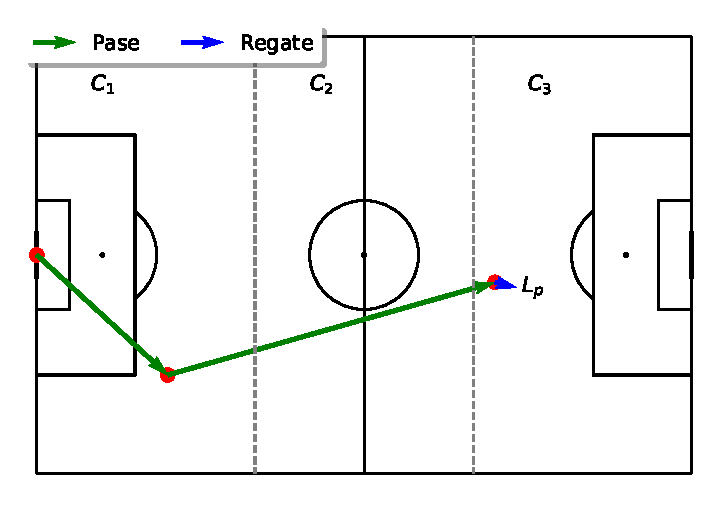
\includegraphics{modelo_files/figure-pdf/cell-2-output-1.pdf}

Para movernos de un estado \(S_i\) a un estado \(S_j\) mediante una
acción \(a_k\) haremos uso de las probabilidades de transición, estas
probabilidades las estimaremos utilizando datos extraídos de
\href{https://fbref.com/es/}{FBREF} para 4 clubes:
\href{https://fbref.com/es/equipos/c02b0f7a/2023-2024/Estadisticas-de-Guadalajara}{Chivas},
\href{https://fbref.com/es/equipos/18d3c3a3/2023-2024/Estadisticas-de-America}{América},
\href{https://fbref.com/es/equipos/632f1838/2023-2024/Estadisticas-de-Cruz-Azul}{Cruz
Azul} y
\href{https://fbref.com/es/equipos/c9d59c6c/2023-2024/Estadisticas-de-Pumas-UNAM}{Pumas}
de la temporada 2023-2024

Primero vamos a interpretar las probabilidades de transición con la
finalidad de descartar aquellas transciones que no serán posibles con
nuestro modelo y con la naturaleza de un partido.

\begin{itemize}
\item
  Fijamos el estado \(C_1\).

  \begin{itemize}
  \item
    Consideramos la acción \(p\):

    \(P(C_1,p,C_1)=\) La probabilidad de estar en la zona \(C_1\) dar un
    \emph{pase} y terminar en la zona \(C_1\).

    \(P(C_1,p,C_2)=\) La probabilidad de estar en la zona \(C_1\) dar un
    \emph{pase} y terminar en la zona \(C_2\).

    \(P(C_1,p,C_3)=\) La probabilidad de estar en la zona \(C_1\) dar un
    \emph{pase} y terminar en la zona \(C_3\).

    \(P(C_1,p,L_p)=\) La probabilidad de estar en la zona \(C_1\) dar un
    \emph{pase} y perder el balón.

    \(P(C_1,p,nG)=\) La probabilidad de estar en la zona \(C_1\) dar un
    \emph{pase} y no anotar gol.

    \(P(C_1,p,G)=\) La probabilidad de estar en la zona \(C_1\) dar un
    \emph{pase} y anotar gol.

    De esta lista de probabilidades para la acción \(p\) notemos que
    \(P(C_1,p,nG)=P(C_1,p,G)=0\) esto pues la única acción admisible
    para terminar en los estados \(\{nG,G\}\) es \(t\).
  \item
    Consideramos la acción \(r\):

    \(P(C_1,r,C_1)=\) La probabilidad de estar en la zona \(C_1\) hacer
    un \emph{regate} y terminar en la zona \(C_1\).

    \(P(C_1,r,C_2)=\) La probabilidad de estar en la zona \(C_1\) hacer
    un \emph{regate} y terminar en la zona \(C_2\).

    \(P(C_1,r,C_3)=\) La probabilidad de estar en la zona \(C_1\) hacer
    un \emph{regate} y terminar en la zona \(C_3\).

    \(P(C_1,r,L_p)=\) La probabilidad de estar en la zona \(C_1\) hacer
    un \emph{regate} y perder el balón.

    \(P(C_1,r,nG)=\) La probabilidad de estar en la zona \(C_1\) hacer
    un \emph{regate} y no anotar gol.

    \(P(C_1,r,G)=\) La probabilidad de estar en la zona \(C_1\) hacer un
    \emph{regate} y anotar gol.

    De esta lista de probabilidades para la acción \(r\) notemos que
    \(P(C_1,r,nG)=P(C_1,r,nG)=0\) esto pues la única acción admisible
    para terminar en los estados \(nG,G\) es \(t\).

    Además \(P(C_1,r,C_3)=0\), pues al realizar un \emph{regate} solo
    tenemos dos opciones:

    nos mantenemos en la zona \(C_1\) o avanzamos a la zona siguiente
    \(C_2\).
  \item
    Consideramos la acción \(t\):

    En este caso tendremos que
    \(P(C_1,t,C_1)=P(C_1,t,C_2)=P(C_1,t,C_3)=P(C_1,t,L_p)=0\) pues
    después de realizar un \emph{tiro} solo tendremos dos estados
    posibles \(\{nG,G\}\).

    \(P(C_1,t,nG)=\) La probabilidad de estar en la zona \(C_1\) hacer
    un \emph{tiro} y no anotar gol.

    \(P(C_1,t,G)=\) La probabilidad de estar en la zona \(C_1\) hacer un
    \emph{tiro} y anotar gol.

    Sin embargo, como suponemos que las acciones que toman las
    futbolistas son razonables, no tiene sentido realizar un \emph{tiro}
    desde la zona \(C_1\), pues la distancia hacia la porteria contaría
    es muy lejana y la probabilidad de anotar un gol es prácticamente
    nula. Por tanto

    \[
      P(C_1,t,S)=0,\hspace{0.5cm}\forall S\in \mathcal{S}.
      \]
  \end{itemize}
\item
  Fijamos el estado \(C_2\).

  \begin{itemize}
  \item
    Consideramos la acción \(p\):

    \(P(C_2,p,C_1)=\) La probabilidad de estar en la zona \(C_2\) dar un
    \emph{pase} y terminar en la zona \(C_1\).

    \(P(C_2,p,C_2)=\) La probabilidad de estar en la zona \(C_2\) dar un
    \emph{pase} y terminar en la zona \(C_2\).

    \(P(C_2,p,C_3)=\) La probabilidad de estar en la zona \(C_2\) dar un
    \emph{pase} y terminar en la zona \(C_3\).

    \(P(C_2,p,L_p)=\) La probabilidad de estar en la zona \(C_2\) dar un
    \emph{pase} y perder el balón.

    \(P(C_2,p,nG)=\) La probabilidad de estar en la zona \(C_2\) dar un
    \emph{pase} y no tirar a gol.

    \(P(C_2,p,G)=\) La probabilidad de estar en la zona \(C_2\) dar un
    \emph{pase} y terminar en gol.

    De esta lista de probabilidades para la acción \(p\) notemos que
    \(P(C_2,p,nG)=P(C_2,p,nG)=0\) esto pues la única acción admisible
    para terminar en los estados \(\{nG,G\}\) es \(t\).
  \item
    Consideramos la acción \(r\):

    \(P(C_2,r,C_1)=\) La probabilidad de estar en la zona \(C_2\) hacer
    un \emph{regate} y terminar en la zona \(C_1\).

    \(P(C_2,r,C_2)=\) La probabilidad de estar en la zona \(C_2\) hacer
    un \emph{regate} y terminar en la zona \(C_2\).

    \(P(C_2,r,C_3)=\) La probabilidad de estar en la zona \(C_2\) hacer
    un \emph{regate} y terminar en la zona \(C_3\).

    \(P(C_2,r,L_p)=\) La probabilidad de estar en la zona \(C_2\) hacer
    un \emph{regate} y perder el balón.

    \(P(C_2,r,nG)=\) La probabilidad de estar en la zona \(C_2\) hacer
    un \emph{regate} y no anotar gol.

    \(P(C_2,r,G)=\) La probabilidad de estar en la zona \(C_2\) hacer un
    \emph{regate} y anotar gol.

    De esta lista de probabilidades para la acción \(r\) notemos que
    \(P(C_2,r,nG)=P(C_2,r,G)=0\) esto pues la única acción admisible
    para terminar en los estados \(\{nG,G\}\) es \(t\).
  \item
    Consideramos la acción \(t\):

    En este caso tendremos que
    \(P(C_2,t,C_1)=P(C_2,t,C_2)=P(C_2,t,C_3)=P(C_2,t,L_p)=0\) pues
    después de realizar un \emph{tiro} solo tendremos dos estados
    posibles \(\{nG,G\}\).

    \(P(C_2,t,nG)=\) La probabilidad de estar en la zona \(C_1\) hacer
    un \emph{tiro} y no anotar gol.

    \(P(C_2,t,G)=\) La probabilidad de estar en la zona \(C_1\) hacer un
    \emph{tiro} y anotar gol.
  \end{itemize}
\item
  Fijamos el estado \(C_3\)

  \begin{itemize}
  \item
    Consideramos la acción \(p\):

    \(P(C_3,p,C_1)=\) La probabilidad de estar en la zona \(C_3\) dar un
    \emph{pase} y terminar en la zona \(C_1\).

    \(P(C_3,p,C_2)=\) La probabilidad de estar en la zona \(C_3\) dar un
    \emph{pase} y terminar en la zona \(C_2\).

    \(P(C_3,p,C_3)=\) La probabilidad de estar en la zona \(C_3\) dar un
    \emph{pase} y terminar en la zona \(C_3\).

    \(P(C_3,p,L_p)=\) La probabilidad de estar en la zona \(C_3\) dar un
    \emph{pase} y perder el balón.

    \(P(C_3,p,nG)=\) La probabilidad de estar en la zona \(C_3\) dar un
    \emph{pase} y no tirar a gol.

    \(P(C_3,p,G)=\) La probabilidad de estar en la zona \(C_3\) dar un
    \emph{pase} y terminar en gol.

    De esta lista de probabilidades para la acción \(p\) notemos que
    \(P(C_3,p,nG)=P(C_2,p,G)=0\) esto pues la única acción admisible
    para terminar en los estados \(\{nG,G\}\) es \(t\).
  \item
    Consideramos la acción \(r\):

    \(P(C_3,r,C_1)=\) La probabilidad de estar en la zona \(C_3\) hacer
    un \emph{regate} y terminar en la zona \(C_1\).

    \(P(C_3,r,C_2)=\) La probabilidad de estar en la zona \(C_3\) hacer
    un \emph{regate} y terminar en la zona \(C_2\).

    \(P(C_3,r,C_3)=\) La probabilidad de estar en la zona \(C_3\) hacer
    un \emph{regate} y terminar en la zona \(C_3\).

    \(P(C_3,r,L_p)=\) La probabilidad de estar en la zona \(C_3\) hacer
    un \emph{regate} y perder el balón.

    \(P(C_3,r,nG)=\) La probabilidad de estar en la zona \(C_3\) hacer
    un \emph{regate} y no anotar gol.

    \(P(C_3,r,G)=\) La probabilidad de estar en la zona \(C_3\) hacer un
    \emph{regate} y anotar gol.

    De esta lista de probabilidades para la acción \(r\) notemos que
    \(P(C_3,r,nG)=P(C_3,r,G)=0\) esto pues la única acción admisible
    para terminar en los estados \(\{nG,G\}\) es \(t\).

    Además \(P(C_3,r,C_1)=0\), pues al realizar un \emph{regate} solo
    tenemos dos opciones o nos mantenemos en la zona \(C_3\) o
    retrocedemos a la zona anterior \(C_2\).
  \item
    Consideramos la acción \(t\):

    En este caso tendremos que
    \(P(C_3,t,C_1)=P(C_3,t,C_2)=P(C_3,t,C_3)=P(C_3,t,L_p)=0\) pues
    después de realizar un \emph{tiro} solo tendremos dos estados
    posibles \(\{nG,G\}\).

    \(P(C_3,t,nG)=\) La probabilidad de estar en la zona \(C_1\) hacer
    un \emph{tiro} y no anotar gol.

    \(P(C_3,t,G)=\) La probabilidad de estar en la zona \(C_1\) hacer un
    \emph{tiro} y anotar gol.
  \end{itemize}
\item
  Por último como \(\{L_p,nG,G\}\) son estados absorbentes, entonces
  \(\forall a\in\mathcal{A}.\)
\end{itemize}

\[
    P(L_p,a,S)=\left\{\begin{array}{ccc}
            1 & \text{si} & S = L_p\\
            0 & o.c. &
            \end{array}\right. 
\]

\[
    P(nG,a,S)=\left\{\begin{array}{ccc}
            1 & \text{si} & S = nG\\
            0 & o.c. &
            \end{array}\right. 
\]

\[
    P(G,a,S)=\left\{\begin{array}{ccc}
            1 & \text{si} & S = G\\
            0 & o.c. &
            \end{array}\right. 
\]

Para facilitar las estimaciones se renombrarán cada probabiidad con los
parámetros que se muestran en las siguientes tablas

\begin{longtable}[]{@{}ll@{}}
\caption{Parámetros para las probabilidades de \(C_1\)}\tabularnewline
\toprule\noalign{}
Probabilidades & Parámetros \\
\midrule\noalign{}
\endfirsthead
\toprule\noalign{}
Probabilidades & Parámetros \\
\midrule\noalign{}
\endhead
\bottomrule\noalign{}
\endlastfoot
\(P(C_1,p,C_1)\) & \(\alpha_{1p}\) \\
\(P(C_1,p,C_2)\) & \(\alpha_{2p}\) \\
\(P(C_1,p,C_3)\) & \(\alpha_{3p}\) \\
\(P(C_1,p,L_p)\) & \(\alpha_{4p}\) \\
\(P(C_1,r,C_1)\) & \(\alpha_{1r}\) \\
\(P(C_1,r,C_2)\) & \(\alpha_{2r}\) \\
\(P(C_1,r,L_p)\) & \(\alpha_{3r}\) \\
\end{longtable}

\begin{longtable}[]{@{}ll@{}}
\caption{Parámetros para las probabilidades de \(C_2\)}\tabularnewline
\toprule\noalign{}
Probabilidades & Parámetros \\
\midrule\noalign{}
\endfirsthead
\toprule\noalign{}
Probabilidades & Parámetros \\
\midrule\noalign{}
\endhead
\bottomrule\noalign{}
\endlastfoot
\(P(C_2,p,C_1)\) & \(\beta_{1p}\) \\
\(P(C_2,p,C_2)\) & \(\beta_{2p}\) \\
\(P(C_2,p,C_3)\) & \(\beta_{3p}\) \\
\(P(C_2,p,L_p)\) & \(\beta_{4p}\) \\
\(P(C_2,r,C_1)\) & \(\beta_{1r}\) \\
\(P(C_2,r,C_2)\) & \(\beta_{2r}\) \\
\(P(C_2,r,C_3)\) & \(\beta_{3r}\) \\
\(P(C_2,r,L_p)\) & \(\beta_{4r}\) \\
\(P(C_2,t,nG)\) & \(\beta_{1t}\) \\
\(P(C_2,t,G)\) & \(\beta_{1t}\) \\
\end{longtable}

\begin{longtable}[]{@{}ll@{}}
\caption{Parámetros para las probabilidades de \(C_3\)}\tabularnewline
\toprule\noalign{}
Probabilidades & Parámetros \\
\midrule\noalign{}
\endfirsthead
\toprule\noalign{}
Probabilidades & Parámetros \\
\midrule\noalign{}
\endhead
\bottomrule\noalign{}
\endlastfoot
\(P(C_3,p,C_1)\) & \(\gamma_{1p}\) \\
\(P(C_3,p,C_2)\) & \(\gamma_{2p}\) \\
\(P(C_3,p,C_3)\) & \(\gamma_{3p}\) \\
\(P(C_3,p,L_p)\) & \(\gamma_{4p}\) \\
\(P(C_3,r,C_2)\) & \(\gamma_{1r}\) \\
\(P(C_3,r,C_3)\) & \(\gamma_{2r}\) \\
\(P(C_3,r,L_p)\) & \(\gamma_{3r}\) \\
\(P(C_3,t,nG)\) & \(\gamma_{1t}\) \\
\(P(C_3,t,G)\) & \(\gamma_{2t}\) \\
\end{longtable}

\bookmarksetup{startatroot}

\chapter{Descripción y Justificación de la
recompensa}\label{descripciuxf3n-y-justificaciuxf3n-de-la-recompensa}

En un partido de fútbol gana el equipo que anota más goles, en caso de
anotar los mismos goles se considera empate y no existe desempate de
ningún tipo.\footnote{No se consideran los partidos de eliminación
  directa donde existe el desempate por penales.} Por lo que la
recompensa será la de anotar un gol \(R=1\), pues es lo único que puede
hacer que un equipo gane un partido. No existe penalización porque los
goles válidos anotados no pueden ser descontandos.

\bookmarksetup{startatroot}

\chapter{Justificación de las
acciones}\label{justificaciuxf3n-de-las-acciones}

Las acciones que puede realizar un equipo durante un partido son
limitadas y se pueden enlistar. Sin embargo para nuestro modelo vamos a
seleccionar las 3 más importantes que son el \emph{pase, tiro} y
\emph{regate}.

\begin{itemize}
\tightlist
\item
  \emph{tiro}: Es la acción que nos permite anotar goles.
\item
  \emph{pase}: Ayuda a un equipo a mover el balón por el campo sin
  necesidad de desplazarse o dejar rivales atrás.
\item
  \emph{regate}: Permite que podamos trasladar el balón de un lugar a
  otro y dejar a rivales atrás.
\end{itemize}

\bookmarksetup{startatroot}

\chapter*{References}\label{references}
\addcontentsline{toc}{chapter}{References}

\markboth{References}{References}

\phantomsection\label{refs}
\begin{CSLReferences}{1}{0}
\bibitem[\citeproctext]{ref-vanroy2}
Van Roy, Maaike, Pieter Robberechts, Wen-Chi Yang, Luc De Raedt, y Jesse
Davis. 2021. {``Leaving goals on the pitch: Evaluating decision making
in soccer''}. \emph{arXiv preprint arXiv:2104.03252}.

\bibitem[\citeproctext]{ref-vanroy1}
Van Roy, Maaike, Wen-Chi Yang, Luc De Raedt, y Jesse Davis. 2021.
{``Analyzing learned markov decision processes using model checking for
providing tactical advice in professional soccer''}. En \emph{AI for
Sports Analytics (AISA) Workshop at IJCAI 2021}.

\end{CSLReferences}




\end{document}
